%%%%%%%%%%%%%%%%%%%%%%%%%%%%%%%%%%%%%%%%%
% Stylish Curriculum Vitae
% LaTeX Template
% Version 1.1 (September 10, 2021)
%
% This template originates from:
% https://www.LaTeXTemplates.com
%
% Authors:
% Stefano (https://www.kindoblue.nl)
% Vel (vel@LaTeXTemplates.com)
%
% License:
% CC BY-NC-SA 4.0 (https://creativecommons.org/licenses/by-nc-sa/4.0/)
%
%%%%%%%%%%%%%%%%%%%%%%%%%%%%%%%%%%%%%%%%%
% !TEX program = xelatex
\documentclass[a4paper, oneside, final, 12pt]{scrartcl} % Paper options using the scrartcl class

\usepackage{fontspec} % for other font
\usepackage{xeCJK} % for chinese font
\usepackage{hyperref} % for hyper web link
\usepackage{multirow} % for tabular table in learning progress
\usepackage{graphicx} % for image insersion
\usepackage[export]{adjustbox} % for image frame
\usepackage{setspace}
\usepackage{array}
% Define typographic struts, as suggested by Claudio Beccari
%   in an article in TeX and TUG News, Vol. 2, 1993.
\usepackage{mathptmx}
\usepackage{scrlayer-scrpage} % Provides headers and footers configuration
\usepackage{titlesec} % Allows creating custom \section's
\usepackage{marvosym} % Allows the use of symbols
\usepackage{tabularx,colortbl} % Advanced table configurations
% \usepackage{ebgaramond} % Use the EB Garamond font
\usepackage{microtype} % To enable letterspacing
\usepackage{pdfpages} % for showing pdf
\usepackage{pdflscape}
\usepackage{enumitem}
\usepackage{subcaption}
\usepackage{listings}   % highlight the python code
\usepackage{xcolor}
\usepackage{multirow}
\usepackage{cite} %Imports biblatex package
\usepackage{amsmath} % for cases command
\usepackage[ruled,linesnumbered]{algorithm2e}
\newcommand\mycommfont[1]{\normalsize\ttfamily\textcolor{blue}{#1}}
\SetCommentSty{mycommfont}
% \usepackage[backend=bibtex,bibencoding=ascii,style=authoryear,sorting=none]{bibtex}
% \addbibresource{reference.bib}
% setup the margin
\usepackage[top=1cm, bottom=1cm, right=2cm, left=2cm]{geometry}

% set the style of listing code
\definecolor{codegreen}{rgb}{0,0.6,0}
\definecolor{codegray}{rgb}{0.5,0.5,0.5}
\definecolor{codepurple}{rgb}{0.58,0,0.82}
\definecolor{backcolour}{rgb}{0.95,0.95,0.92}

\lstdefinestyle{mystyle}{
    backgroundcolor=\color{backcolour},   
    commentstyle=\color{codegreen},
    keywordstyle=\color{magenta},
    numberstyle=\tiny\color{codegray},
    stringstyle=\color{codepurple},
    basicstyle=\ttfamily\footnotesize,
    breakatwhitespace=true,         
    breaklines=true,                 
    captionpos=b,                    
    keepspaces=true,                 
    numbers=left,                    
    numbersep=5pt,                  
    showspaces=false,                
    showstringspaces=false,
    showtabs=false,                  
    tabsize=2
}

\lstset{style=mystyle}

% set chinese and english font
\setmainfont{Times New Roman}
\setCJKmainfont[AutoFakeBold=true, AutoFakeSlant=true]{標楷體}

\titleformat{\section}{\Large\raggedright\bfseries}{}{0em}{}[\titlerule] % Section formatting
\titleformat{\subsection}{\large\raggedright\bfseries}{}{0em}{}
\titleformat{\subsubsection}{\normalsize\raggedright\bfseries}{}{0em}{}

% \pagestyle{scrheadings} % Print the headers and footers on all pages

% enable bold and slant chinese font
% \xeCJKsetup{AutoFakeBold=true, AutoFakeSlant=true}

% set the space at the front of paragraph
\setlength{\parindent}{2em}

% disable page number
\pagenumbering{gobble}

\newcommand{\gray}{\rowcolor[gray]{.90}} % Custom highlighting for the work experience and education sections
\newcommand{\Tstrut}{\rule{0pt}{2.6ex}}         % = `top' strut
\newcommand{\Bstrut}{\rule[-0.9ex]{0pt}{0pt}}   % = `bottom' strut
\newcommand{\Tstruth}{\rule{0pt}{4ex}}         % = `top' strut for header
\newcommand{\Bstruth}{\rule[-2.5ex]{0pt}{0pt}}   % = `bottom' strut for header

%----------------------------------------------------------------------------------------
%	FOOTER SECTION
%----------------------------------------------------------------------------------------

% \renewcommand{\headfont}{\normalfont\rmfamily\scshape} % Font settings for footer

% \cofoot{
% \fontsize{12.5}{17}\selectfont % Letter spacing and font size

% \textls[150]{123 Broadway {\large\textperiodcentered} City {\large\textperiodcentered} Country 12345}\\ % Your mailing address
% {\Large\Letter} \textls[150]{john@smith.com \ {\Large\Telefon} (000) 111-1111} % Your email address and phone number
% }

%----------------------------------------------------------------------------------------
\begin{document}

%----------------------------------------------------------------------------------------
%	HEADER SECTION
%----------------------------------------------------------------------------------------


\begin{center}
    {\fontsize{18}{30}\textbf{Game Theory HW2 \\ Graph Problem}}
\end{center}

\begin{center}
  Bo-Han Chen (陳柏翰) \\
  Student ID:312551074 \\
  bhchen312551074.cs12@nycu.edu.tw
\end{center}

\section{Experiment Environment}

\begingroup
\raggedright

\begin{itemize}
  \item OS: Windows 10 22H2
  \item Hardware: Intel(R) Xeon(R) CPU E3-1231 v3 @ 3.40GHz
  \item Python 3.12.0
  \begin{itemize}
    \item networkx 3.2.1
    \item matplotlib 3.8.0
  \end{itemize}
\end{itemize}

\section{Requirement 1-1: Weighted MIS Game}

\subsection{Problem Statement}

The goal of Weighted MIS Game is to maximize the total weight in the MIS set.
In my implementation, the following function used to 
determine the priority of nodes is shown below:
$$PR_i = \frac{W(p_i)}{W(p_i) + \sum_{p_j \in N_i}{W(p_j)}}$$
For each player, the utility function is defined as:
$$u_i(C) = \sum_{p_j \in L_i} \omega(c_i, c_j) + c_i$$
where
$$\omega(c_i, c_j) = -\alpha c_i c_j, \alpha > 1$$
and
$$L_i = \{ p_j|p_j \in N_i \wedge PR_i \le PR_j \}$$
From the ultility function shown above, we can see the player will prefer to
join the MIS set if there are no neighbor with higher priority in the set, 
which lead to the best response shown below:
$$BR_i(C_{-i}) = 
\begin{cases}
  0, & \text{if } \exists p_j \in L_i, c_j = 1 \\
  1, & \text{otherwise.}
\end{cases}$$

\subsection{Code Description}

For the implementation of this assignment, I use \emph{networkx} library's \emph{Graph}
structure to represent the graph.
After parsing the command-line arguments, 
the constructor of \emph{gameModel} will take the number of nodes, 
the edge list, the type of game and the times of simulation as input.

\lstinputlisting[language=Python, caption=Constructor of gameModel,
                  label = {lst:Constructor of gameModel}]
                  {./ref_code/gameModel Constructor.py}

Then the \emph{init\_graph} function will be called to 
initialize the nodes and edges of \emph{Graph}.

\lstinputlisting[language=Python, caption=Graph Initialization,
                  label = {lst:Graph Initialization}]
                  {./ref_code/Graph Initialization.py}

To initialize the weight, priority and strategy of nodes in weighted MIS game, 
the \emph{init\_node\_MIS} function will be called.The weight is set as the node id, 
and the initial strategy of each node will be randomly
selected from the strategy set $\{0, 1\}$.

\lstinputlisting[language=Python, caption=Node Initialization of Weighted MIS Game,
                label = {lst:Node Initialization of Weighted MIS Game}]
                {./ref_code/MIS node Initialization.py}

The simulation of Weighted MIS Game is shown in Listing \ref{lst:Weighted MIS Game}.
For each iteration, each node will be checked to see 
if it can get higher utility.
If there are multiple nodes perfer to change their strategy,
one of them will be randomly selected and change its strategy to best response.
If there are no nodes will change their strategy, 
the simulation will be terminated since the NE is reached.
The cardinality of the MIS set (the number of nodes in the MIS set) 
will be returned as the result.

\lstinputlisting[language=Python, caption=Weighted MIS Game, 
                 label={lst:Weighted MIS Game}]
                {./ref_code/Weighted MIS Game.py}

\subsection{Experiment Result}

The graph of test case is shown in Figure \ref{fig:Test Case Graph}:

\begin{figure}[h]
  \centering
  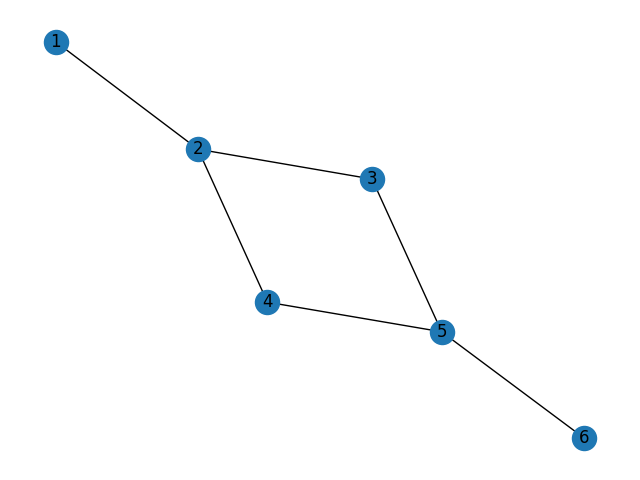
\includegraphics[width=0.6\textwidth]{./image/original_graph.png}
  \caption{Test Case Graph}
  \label{fig:Test Case Graph}
\end{figure}

The result of Weighted MIS Game is shown in Figure \ref{fig:Result of Weighted MIS Game},
the node in the MIS set is colored in blue, and the red one is not in the MIS set.
With the test case, we can see the result is correct since the total weight of MIS set
is the maximum value, 14.

\begin{figure}[h]
  \centering
  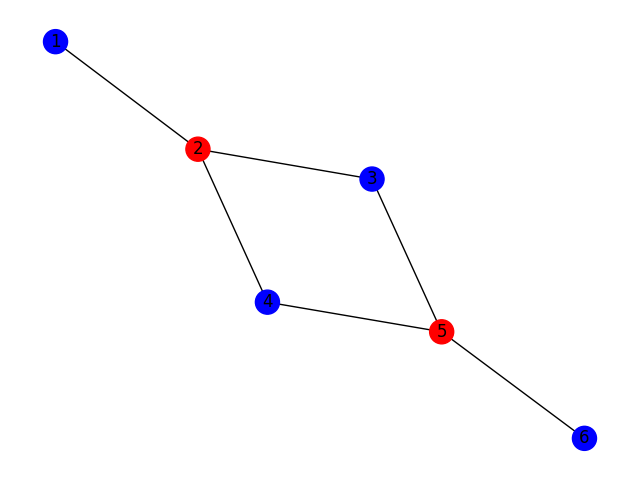
\includegraphics[width=0.6\textwidth]{./image/result_weighted_mis.png}
  \caption{Result of Weighted MIS Game}
  \label{fig:Result of Weighted MIS Game}
\end{figure}
\section{Requirement 1-2: Symmetric MDS-based IDS Game}


\subsection{Problem Statement}

By the definition of utility function in the slides:
$$u_i(C)=
\begin{cases}
  \left(\sum_{p_j \in M_i}{g_j(C)}\right) - \beta - \omega_{i}(C) & \text{if } c_i = 1 \\
  0 & \text{otherwise.}
\end{cases}
$$

We can know that the player will prefer to join the IDS set 
only if all following conditions are satisfied:
\begin{enumerate}
  \item Avoid violating the independence rule: All of its' neighbors are not in the IDS set 
  (the player itself is not dominated).
  \item Gain of dominance: At least one of its' neighbors ($p_j$) is not 
  dominated by players in set $N_j \cup \{p_j\}$.
\end{enumerate}

So the best response of each player is shown below:
$$
BR_i(C_{-i}) =
\begin{cases}
  0, & \text{if } \left(\exists p_j \in N_i, c_j = 1\right) \text{ or } 
  \left( \forall p_j \in N_i, v_j(c_{-i}) \ge 1 \text{ and } 
  \sum_{p_j \in N_i}{c_j} \ge 1 \right) \\
  1, & \text{otherwise.}
\end{cases}
$$
where
$$v_i(C) = \sum_{p_j \in M_i}{c_j}, M_i = N_i \cup \{p_i\}$$

\subsection{Code Description}

The simulation of Symmetric MDS-based IDS Game is shown in 
Listing \ref{lst:Symmetric MDS-based IDS Game}.
Like the implementation of previous section,
nodes that can get higher utility will be randomly selected and change their strategy.
First the independence rule will be checked to see 
if there is any neighbor is already in the IDS set.
If so, the node will choose to leave the IDS set to avoid the panelty  of violating the rule.
Then we check whether the node itself is dominated by any of its' neighbors, 
why we not check the strategy of node itself is because
the node will choose to leave the IDS set even if it is only dominated by itself, 
which leads to the wrong result.
After checking the dominance of neighbors,
if the node and all of its' neighbors are already dominated,
the node will choose to leave the IDS set since it can not get any gain of dominance
(which leads to $-\beta$ utility).

When reaching NE, the cardinality of IDS (number of nodes in IDS set) will be returned.

\lstinputlisting[language=Python, 
  caption=Symmetric MDS-based IDS Game, label={lst:Symmetric MDS-based IDS Game}]
  {./ref_code/Symmetric MDS-based IDS Game.py}

\subsection{Result and Discussion}

For the provided test case, the cardinality of IDS set might be 2 or 4.
The result is shown in Figure \ref{fig:Result of Symmetric MDS-based IDS Game}.

\begin{figure}[h]
  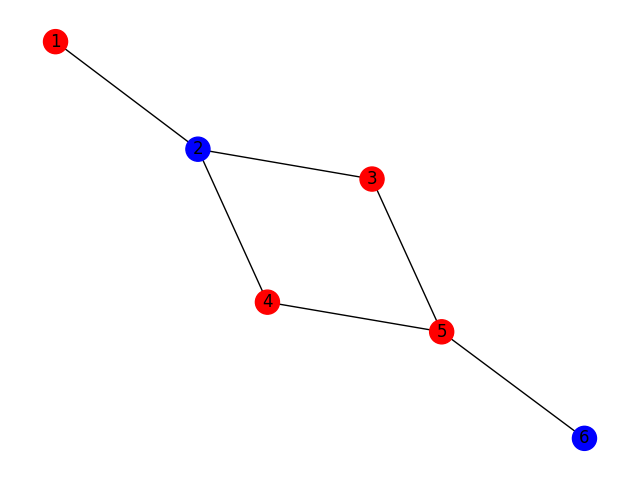
\includegraphics[width=0.5\textwidth]{./image/result_ids_2.png}
  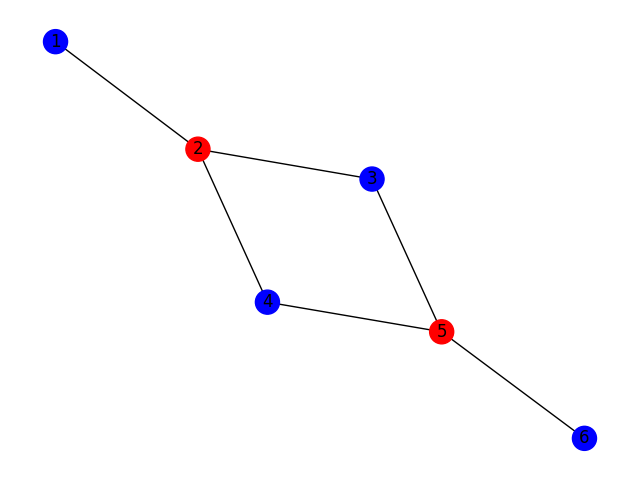
\includegraphics[width=0.5\textwidth]{./image/result_ids.png}
  \caption{Result of Symmetric MDS-based IDS Game}
  \label{fig:Result of Symmetric MDS-based IDS Game}
\end{figure}

We can see that some result of Symmetric MDS-based IDS Game is not the best NE,
the reason is that the simulation is initialized with random strategy,
and for each iteration, the node that can change the strategy is selected randomly.
To ensure the result of Symmetric MDS-based IDS Game is the best NE,
I set the running times of simulation to 300000 and record the minimum cardinality of IDS set.

\section{Requirement 2: Matching Game}

\subsection{Problem Statement}

In the matching game, each node will find the neighbor that is unmatched form a pair.
In order to increase the number of matched pairs,
each node will be assigned a priority based on its degree initially,
and the node with higher priority will be prefered to form a pair.
For the matching game, the utility function of each player can be defined as
($H_i$ represents the set of higher priority neighbors,
and $L_i$ represents the set of lower priority neighbors):
$$u_i(C) = 
\begin{cases}
  \alpha, & \text{if } c_i = p_j \text{ and } c_j = p_i, p_j \in H_i \\
  \beta,  & \text{if } c_i = p_j \text{ and } c_j = null, p_j \in H_i \\
  \gamma, & \text{if } c_i = p_j \text{ and } c_j = p_i, p_j \in L_i \\
  \delta, & \text{if } c_i = p_j \text{ and } c_j = null, p_j \in L_i \\
  \epsilon, & \text{if } c_i = null \\
  0, & \text{if } c_i = p_j \text{ and } c_j = p_k, p_k \in N_j \setminus \{p_i, null\} \\
\end{cases}
$$
where
$$ \alpha > \beta > \gamma > \delta > \epsilon > 0$$
and
\begin{gather*}
  H_i = \{p_j | p_j \in N_i \land PR_j > PR_i\} \\
  L_i = \{p_j | p_j \in N_i \land PR_j \le PR_i\} \\
  PR_i = \frac{1}{deg(p_i)}
\end{gather*}

With the utility function above, we can define the best response of each player as(
$HM_i$ represents the set of higher priority neighbors that match the node,
$HN_i$ represents the set of higher priority neighbors that not choose any nodes,
$LM_i$ represents the set of lower priority neighbors that match the node,
$LN_i$ represents the set of lower priority neighbors that not choose any nodes
):
$$ BR_i(C_{-i})=
\begin{cases}
  p_j, & p_j \in HM_i, \text{if } HM_i \ne \emptyset \\
  p_k, & p_k \in HN_i, \text{if } HM_i = \emptyset \land HN_i \ne \emptyset \\
  p_l, & p_l \in LM_i, \text{if } HM_i \cup HN_i = \emptyset \land LM_i \ne \emptyset \\
  p_m, & p_m \in LN_i, \text{if } HM_i \cup HN_i \cup LM_i = \emptyset \land LN_i \ne \emptyset \\
  null, & \text{otherwise.}
\end{cases}
$$
where
\begin{gather*}
HM_i = \{p_j | p_j \in H_i \land c_j = p_i\} \\
HN_i = \{p_j | p_j \in H_i \land c_j = null\} \\
LM_i = \{p_j | p_j \in L_i \land c_j = p_i\} \\
LN_i = \{p_j | p_j \in L_i \land c_j = null\} \\
\end{gather*}

If there are neighbor with higher priority tend to form a pair with the node,
the node will first choose it to form a pair, 
if there are no such neighbor, 
the node will choose the high-priority neighbor that are not choosing any node.
If the node cannot match any high-priority neighbor,
it will try to match the low-priority neighbor with the same condition mentioned above.
Finally, if the node cannot match any neighbor, it will choose to be unmatched.

\subsection{Code Description}

The simulation of Matching Game is shown in Listing \ref{lst:Matching Game}.
Before the simulation, the strategy of each node will be randomly selected from the set
including its' neighbors and 0 (unmatched),
and the priority of each node will be calculated based on its degree.
For each iteration, each node will be checked to see
if it can get higher utility.
If there are nodes perfer to change their strategy,
\emph{candidate\_nodes} will store two list including the nodes and its best response.
Then one of the nodes will be randomly selected and change its strategy to best response.
Finally, the cardinality of the matched pairs will be returned as the result.

\lstinputlisting[language=Python, 
  caption=Matching Game, label={lst:Matching Game}]
  {./ref_code/Matching Game.py}

\subsection{Result and Discussion}

The result of Matching Game simulated on the provided test case 
is shown in Figure \ref{fig:Result of Matching Game}.

\begin{figure}[h]
  \centering
  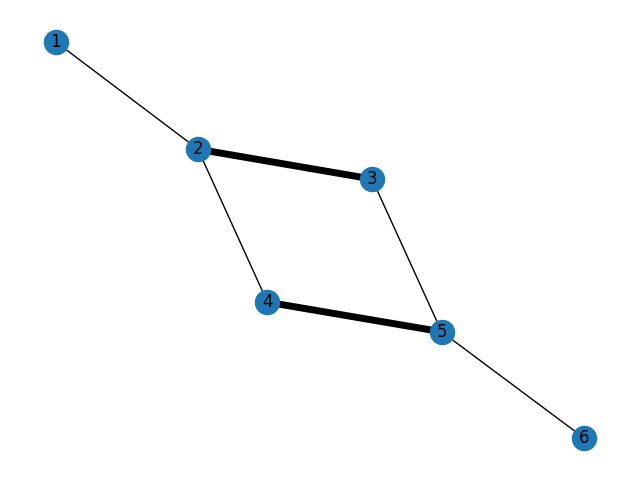
\includegraphics[width=0.45\textwidth]{./image/result_match_game.png}
  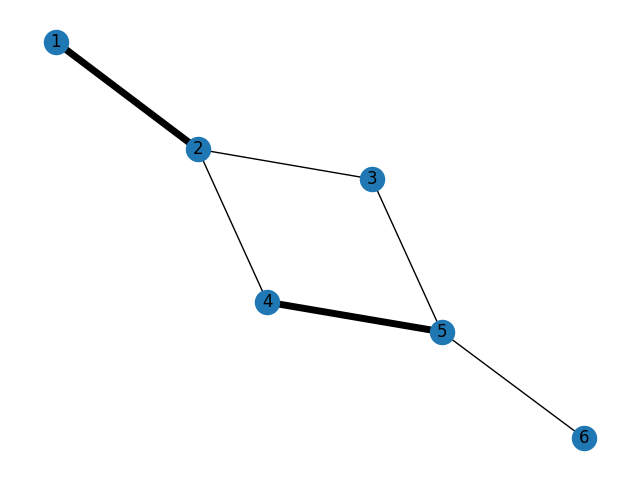
\includegraphics[width=0.45\textwidth]{./image/result_match_game_2.png}
  \caption{Some Result of Matching Game}
  \label{fig:Result of Matching Game}
\end{figure}

For the test case, the cardinality of Matching Game is always the maximal and maximum, 2.
To verify if there are any situation that the cardinality of simulation is not maximum,
I try another test case shown in Figure \ref{fig:Another Test Case Graph}.

\begin{figure}[h]
  \centering
  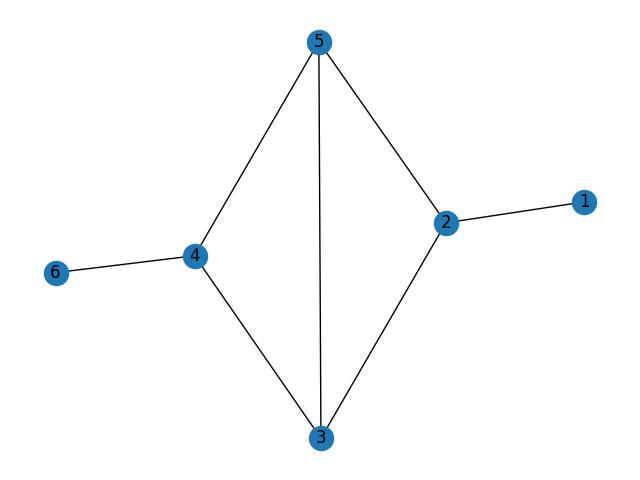
\includegraphics[width=0.6\textwidth]{./image/original_graph_2.png}
  \caption{Test Case 2  for Matching Game}
  \label{fig:Another Test Case Graph}
\end{figure}

The result of Matching Game is shown in Figure \ref{fig:Result of Matching Game 2}.

\newpage

\begin{figure}[h]
  \centering
  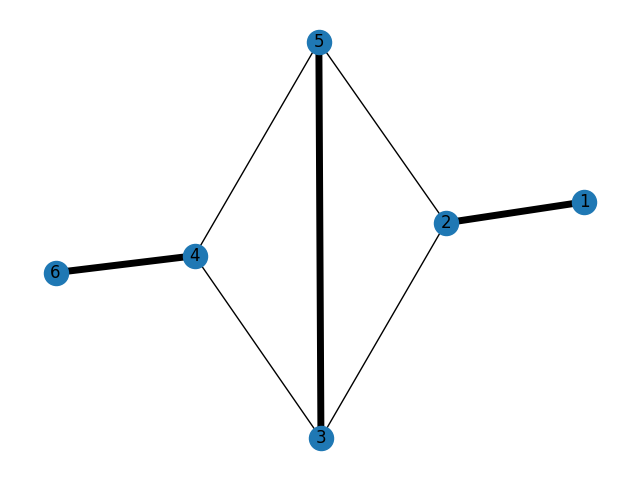
\includegraphics[width=0.45\textwidth]{./image/result_match_game_other.png}
  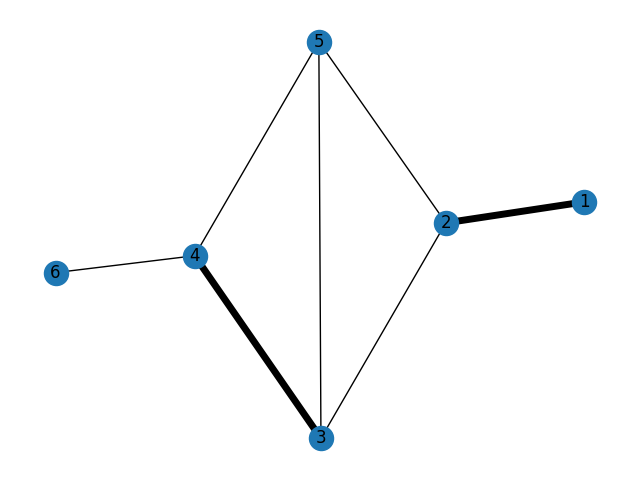
\includegraphics[width=0.45\textwidth]{./image/result_match_game_other_2.png}
  \caption{Result of Matching Game 2}
  \label{fig:Result of Matching Game 2}
\end{figure}

As we can see, the cardinality of Matching Game is not always the maximum,
for the result on the right, the cardinality is 2, which is maximal but not maximum.
The reason is the same as mensioned in the previous section,
with the random strategy initialization and random selection of nodes to change strategy,
the result of simulation is not always the best NE.
In Matching Game simulation, I set the running times of simulation to 10000 get record the maximum cardinality
to ensure the result is the best NE.

\endgroup

\end{document}